\documentclass[11pt,a4paper]{article}
\usepackage[utf8]{inputenc}
\title{Preparatório 11 - Eletrônica}
\author{Hiago Riba Guedes RGU:11620104}
\date{Professor:Guilherme Garcia}
\usepackage{tikz}
\usepackage{circuitikz}
\usepackage{graphicx}
\usepackage{amsmath}
\usetikzlibrary{arrows,shapes,positioning,mindmap,trees,automata}
\usepackage{subfigure}
\graphicspath{{/home/hiago/Desktop/}}

\begin{document}
\maketitle
\begin{center}
$ {\begin{array}{cc}
   V_{CE}=7 V &R_{C}=220 \Omega     \\
   V_{E}=1.5 V & Transistor BD19 \\
   V_{BE}=0.7 V & I_{B}=230 uA    \\
   I_{C}=32 mA   \\
  \end{array} } $
   \end{center}
\textbf{4.1-}\\
\\
$V_{CC}=V_E+V_{CE}+R_CI_C$=1,5+7+220.32.10$^{-3}$=15.54 V
\\\\
\textbf{4.2-}\\\\
$\frac{V_E}{I_C}=\frac{1.5}{32 \times 10^{-3}}=46.875 \Omega$
\\\\
\textbf{4.3-} 
\\\\
$V_B=V_{BE}+V_E=2.2 V$\\

Retirando-se o raciocínio do livro(Dispositivos Eletrônicos e teoria de circuitos,8ª edição , Robert L. Boylestad,Louis Nashelsky,Exemplo 4.10,página 132 ) , presume-se que para o circuito funcione eficientemente presume-se que as correntes de $R_1$ e $R_2$ devam ser aproximadamente iguais e muito maiores que a corrente de base(no mínimo 10:1).Ou seja:\\\\
$R_2 \le \frac{1}{10}\times\beta \times R_E$\\
$V_B=\frac{R_2}{R_1 + R_2}\times V_{cc}$\\
$R_2=\frac{1}{10}\times(140)\times(\frac{1.5}{32mA})$\\
$R_2=656.25 \Omega$\\
$2.2=\frac{656.25}{R_1+656.25}\times 15.54$\\\\
Fazendo o cálculos achamos $R_1=3.98 \Omega$
\\\\\\\\\\\textbf{4.4-}\\\\
$\beta=140$\\
$r_o=42 K\Omega$\\
Ganho de corrente=$\beta$=140\\
%Impedância de entrada=$\frac{1}{2\pi fC_s}$\\\\
Modelo usado para o transistor: \\\\
\begin{circuitikz}
\draw(0,0) to[short,o-,i>=$I_b$](1,0)to[R=$R_\pi$](1,-2)to[short](5,-2)to[R=$R_o$,-*](5,0)to[short,-o,i<=$I_c$](6,0);
\draw(5,0)to[short](3.5,0)to[american controlled current source](3.5,-2);
\draw(2,-2)to[short,*-o](2,-2.5);
\node[below right] at(0,0){b};
\node[above left]at (2,-2.5){e};
\node[below right]at(6,0){c};
\end{circuitikz}\\
Onde $r_\pi$ é a impedância de entrada.Que é calculada pela seguinte fórmula:\\
$\beta \times i_b=(\frac{\beta}{r_{\pi}})V_{BE}$\\
$140 \times 230\times10^{-6}=\frac{140}{r_\pi}\times 0.7$\\
Impedância de entrada=3043.48$\Omega$\\\\
Impedância de saída é igual ao $r_o$ que foi dado e é $42 k\Omega$\\
Ganho de tensão é $\frac{V_{CE}}{V_{BE}}=\frac{7}{0.7}=10$
\\\\
\textbf{4.5-}\\

Pelo datasheet do transistor BD-139 vemos que $I_c$ de saturação é igual a 500 mA e para tal temos $I_B$ de 50 mA e $V_{CEsat}=0.5 V$ \\\\
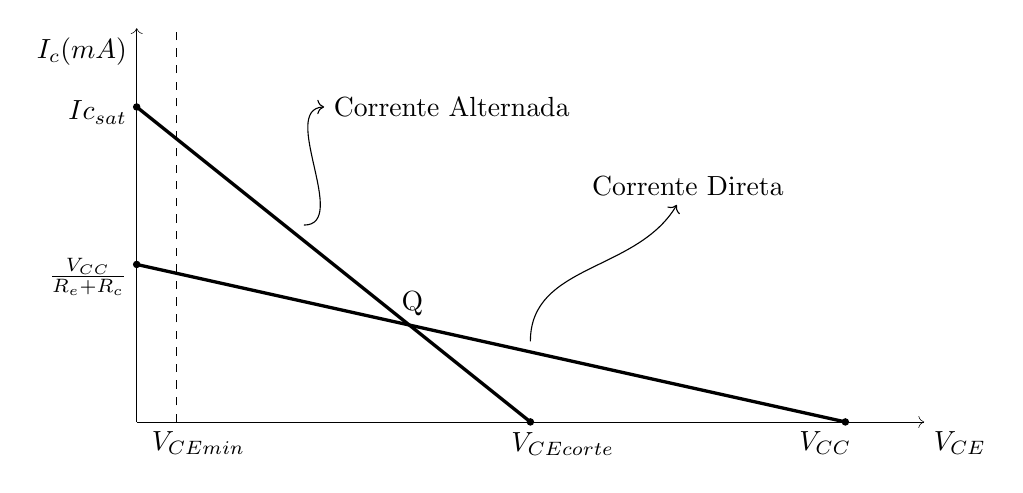
\begin{tikzpicture}
\draw[very thin,->] (0,0)--(0,5);
\draw[very thin,->] (0,0)--(10,0);
\node[below left] at (0,5){$I_c(mA)$};
\node[below right] at (10,0){$V_{CE}$};
\draw[dashed] (0.5,0)--(.5,5);
\node[below left]at(1.5,0){$V_{CEmin}$};

\draw[fill=black] (0,4) circle (.04);
\node[below left] at(0,4.2){$Ic_{sat}$};
\draw[fill=black] (5,0) circle (.04);
\node[below left,very thick] at(6.2,0){$V_{CEcorte}$};
\draw[very thick] (0,4)--(5,0);

\draw[fill=black] (0,2) circle (.04);
\node[below left] at(0,2.2){$\frac{V_{CC}}{R_e+R_c}$};
\draw[fill=black] (9,0) circle (.04);
\node[below left] at(9.2,0){$V_{CC}$};
\draw[very thick] (0,2)--(9,0);

\node (A) at (2,2.5){};
\node (B) at (4,4){Corrente Alternada};
\node (C) at(5,0.9){};
\node (D) at(7,3){Corrente Direta};

 %\draw[->,rounded corners] (A) |- (B);
 \draw[->] (A) to[out=0,in=180] (B);
 \draw[->] (C) to[out=90,in=240] (D);
 \node at(3.5,1.5){Q};
\end{tikzpicture}

Explicação que vejo mais sensata é por que como para DC temos a limitação dos resistores para a corrente no emissor , nós devemos ficar um pouco acima do ponto Q pra não ter problema de entrar na região de corte.
\end{document}